\chapter{Protocol Implementation}
\label{chap:protocolimplementation}

This chapter details the simulation environment where the presented High Configurable Protocol was developed and tested. Simulation was chosen 
instead of analytical study or real networks, because this are difficult or expensive for such a complex protocol. During this chapter a 
deeper view into the protocol will be given, as all generated code will be explained in detail.

\section{Used Tools}

To develop this project different simulators and frameworks for this simulators where considered, choosing finally \ac{OMNeT++} 4.0 \cite{OMNeT}
as simulator, and \ac{MiXiM} 2.0 \cite{MiXiM} as framework, due to its versatility, their short time to get to work with them for the first time and 
their current development of 802.15.4 standard, specially in non-beaconed mode.

After all simulations are done, the results are extracted with a tool called \textit{scavetool}. This data is than imported and treated with 
\ac{MATLAB} \cite{MATLAB} to obtain all results in shown Chapter \ref{chap:simulationandresults}: \nameref{chap:simulationandresults}.

\subsection{\ac{OMNeT++} 4.0}

\ac{OMNeT++} 4.0 is an object oriented discrete event simulator, based in C++ \cite{cpp}. \ac{OMNeT++} consists in several modules hierarchically
connected and that communicate among them through messages. Modules relation is done through an own easy programming language called \ac{NED}.
This language is used in the \textit{.ned} files, which apart from relations among modules, contain parameters about them. The value for this
parameters can be given directly in the \textit{.ned} file or also in a file called \textit{omnetpp.ini}, that is the network configuration file.
This file's content is basically simulation configuration parameters and module parameter values.

This software allows two kind of simulation environments, a graphic one (Tkenv) and a command line one (Cmdenv). Working with the graphic one, 
message interchange simulation can be done step by step, this mode is good to debug the code. The command environment, allows to
make express simulations to obtain faster the final results, in this mode it is also possible to program some
parameter changes during the simulation and also some consecutive simulations, this is all automatically done and thus does not require user 
intervention. This mode makes all process much easier when lots of iterations must be done. When random numbers are generated, they depend on 
a seed. \ac{OMNeT++} changes this seed usually with the run number, making possible that the same run make the same results,
this is very useful in debugging process.

All modules in \ac{OMNeT++} are executed theoretically in a concurrent way, usually computers have only one processor so this is not always
practically possible. Anyway, from here it should be extracted that when a module depends on other module's data, the data should be taken at a 
later moment, if it is done at the same moment, data might not be ready.

All \ac{OMNeT++} modules have the same structure as they inherit all from the same class \textit{cSimpleModule}, later on, some modules could 
implement new methods, but they all have this basic ones:

\begin{itemize}
 \item \textbf{initialize - }This method is executed in every module at the beginning of the simulation and only there (time T = 0).
This method gets as parameter \textit{stage} and it is called by the \ac{OMNeT++} core. This parameter goes from 0 until the number defined with 
method \textit{numInitStages()}.

Before, it was said that all modules in \ac{OMNeT++} are executed concurrently, this means that if it is needed to initialize the network in 
an specific order, this should be done separating code among all the stage phases, as first all stages 0 will be executed, then all stages 1, 
and so on until the number defined for each module. This way data dependencies between modules at initialization can be solved. At least a 
message should be send in this phase, otherwise, the network will not start doing anything.
 \item \textbf{finalize - }This method is in charge of storing all the variables desired to have as results at the simulation end. Here variables
should not be deleted, that should be done in the class destructor.
 \item \textbf{handleMessage - }This method is the one executed each time a message arrives to a module. All modules are connected through gates,
being in this work usually the ones showed in Figure \ref{fig:omnetmodule}. Messages arrived to a module could come from one of the gates or being a self
message. Usually this method calls another methods that take care of the message depending if it is a self message (usually used to schedule 
tasks in a future time), a data message or a control message. This methods are: \textit{handleSelfMsg, handleUpperMsg, handleLowerMsg, 
handleLowerControl and handleUpperControl}.
\begin{figure}[ht]
 \begin{center}
  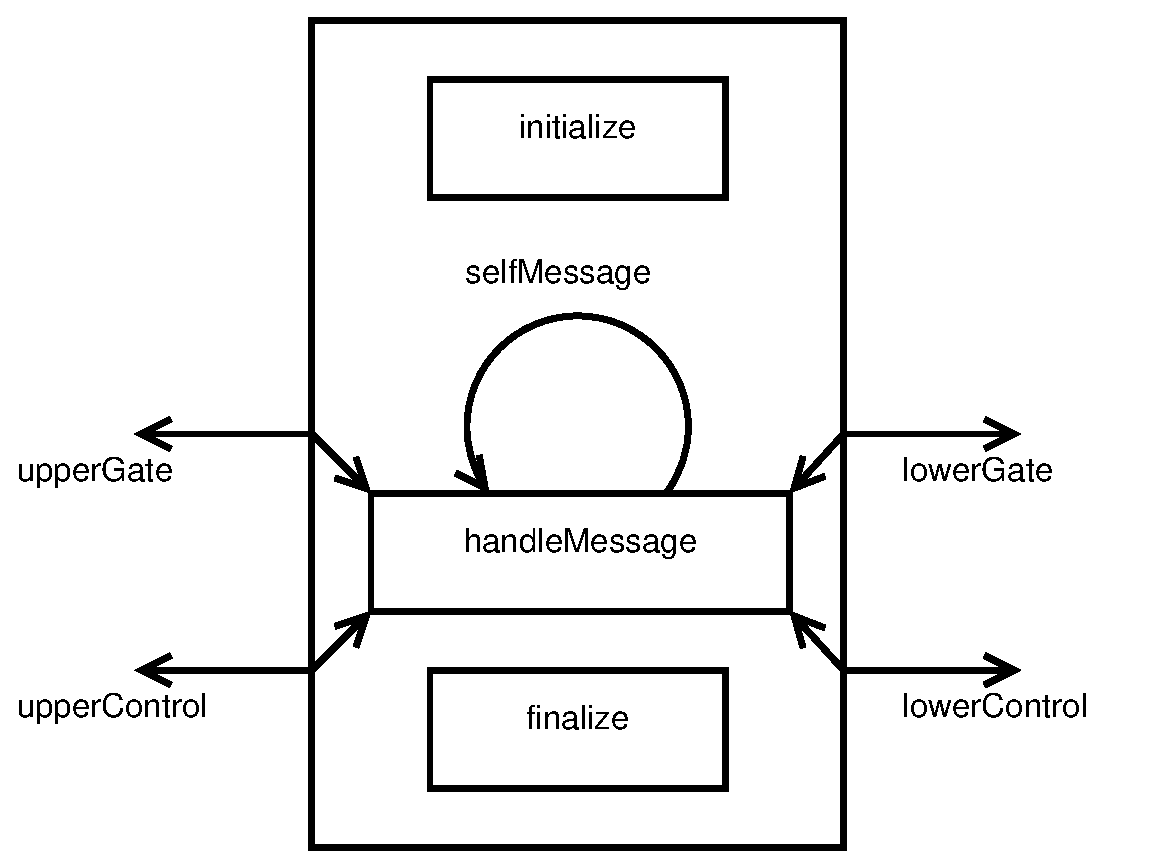
\includegraphics[width=0.5\textwidth]{omnetmodule.eps}
 \end{center}
 \caption{Basic \ac{OMNeT++} module structure}
 \label{fig:omnetmodule}
\end{figure}
 \item \textbf{sendDown/sendUp/sendControlDown/sendControlUp }This methods send a message from a module through the already commented gates.
 \item \textbf{scheduleAt - }As the name says, it schedules a self message in a certain time in the future.
 \item \textbf{decapsMsg/encapsMsg - }Usually before a message is sent from one layer in a device to another, it should be encapsulated or 
decapsulated. When this is done, instead of message, it is talked about a packet. Packet is a class that inherits from class message. It is 
also possible to define a custom packet.
\end{itemize}

This methods were commented here because they are going to be used many times during the work. For more information about \ac{OMNeT++}, 
refer to the user manual \cite{manualomnet}.

\subsection{\ac{MiXiM} Framework}

\ac{MiXiM} 2.0 framework provides \ac{OMNeT++} with many new modules. Among them, all necessary modules to work with 802.15.4 Standard. 
All this modules are build following \cite{IEEE802.15.4-2006}.

The basic structure of a node in \ac{MiXiM} is like shown in Figure \ref{fig:miximmodule}. This figure shows already some new modules added by
this work to the basic \ac{MiXiM} node. Depending on the kind of node: Computer, \ac{AN} or \ac{MN}, the \textit{.ned} files will load 
different modules to describe each behavior.

\begin{figure}[ht]
 \begin{center}
  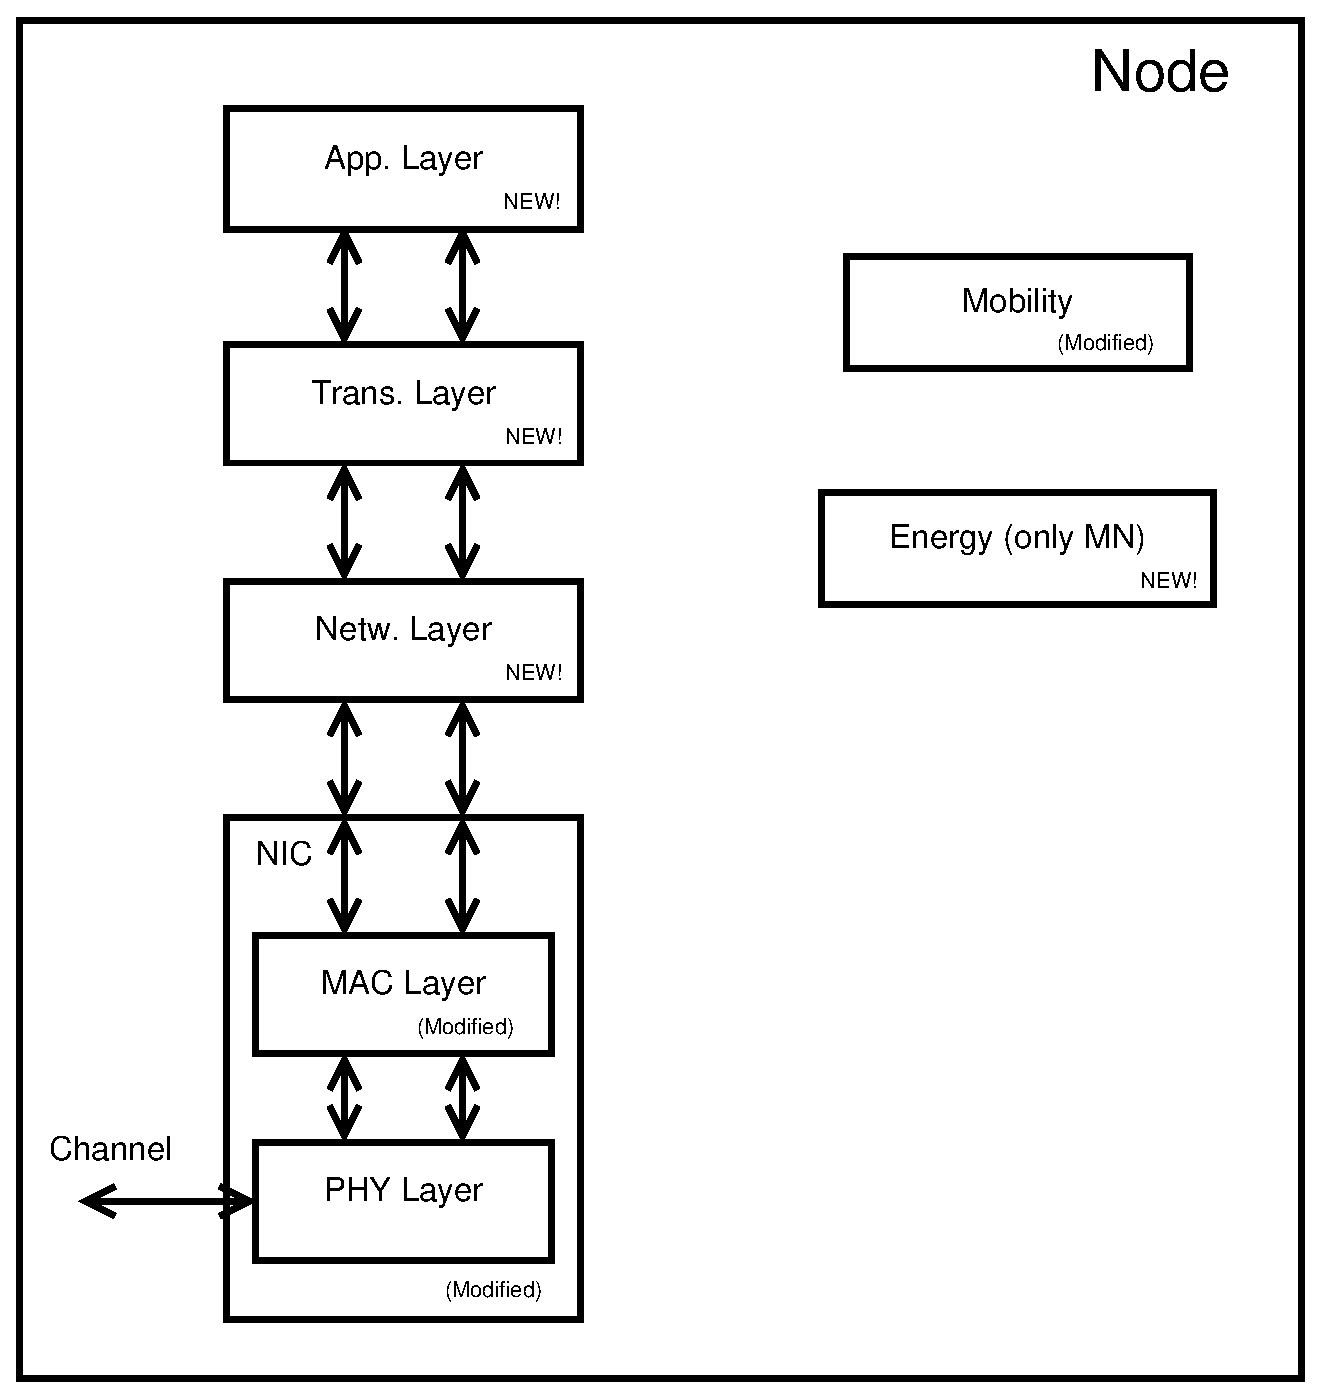
\includegraphics[width=0.6\textwidth]{miximmodule.eps}
 \end{center}
 \caption{Basic \ac{MiXiM} node structure}
 \label{fig:miximmodule}
\end{figure}

Apart from node structure modules, there is a central module in \ac{MiXiM}, called \textit{connectionManager}, in charge of connecting
all nodes at a reachable distance. This module keeps a list of all nodes and it is called every time a node changes its position to
update the position in the list and recalculate all connections. The maximum distance where two nodes could still reach each other, is 
calculated using the transmit power and sensitivity, both defined in \textit{omnetpp.ini}.

In this sub-section, only modified \ac{MiXiM} original modules will be commented leaving the new implemented modules for the next sub-sections.

\subsubsection{Connection Manager}

Comentar aqui tambien los cambios en NicEntry

\subsubsection{Mobility module modifications}

\subsubsection{\ac{MAC} Layer modifications}

Hablar algo sobre los mensajes .msg y para que se usan y que parametros he anadido

When we disabled the CSMA, we have to add a LIFS time to respect the standard time between the end of transmision of a packet to the beggining of the next packet. This time was previously not necesary as the first backoff time was bigger.


\section{Sync Phase study development}

Before constructing all the protocol framework, it had to be decided if during the Sync Phase the \acp{AN} would transmit synchronized in 
slots or randomly. For this purpose, it was done a special small framework where just the Application Layer was added to the nodes.


\subsection{\ac{MN}}

El nodo movil solo contaba el numero de paquetes recibidos en App

\subsection{Computer}

Solo calcula los slots

\subsection{\ac{AN}}

Los anchor generaban los paquetes de forma aleatoria esperando maximo 6 segundos (param definido en omnetpp.ini) y un maximo de paquetes tambien 
definido, o tambien los paquetes que les de tiempo en una segunda fase.

Cuando era con slots explicar el calculo de los slots y luego el tiempo que resultaba de este calculo para 3 veces por sync phase era el que se 
usaba en transmisiones aleatorias para ver cuantos paquetes daba tiempo en este tiempo.


\section{Framework development}

Comentar que el routing es fijo para facilitarlo y hablar de la estructura de grid y del enrutamiento.
